\documentclass[UTF8]{ctexart}

\usepackage{WeeklyReport}
\usepackage{graphicx}
\usepackage{amsmath}
\usepackage{amssymb}

\title{周报20200927}
\author{Jeff Fu}
\date{\today}

\begin{document}
\maketitle
% \tableofcontents
\section{本周计划}
\begin{itemize}
    \item MSDA 论文阅读(Domain Adaptive Ensemble Learning)
\end{itemize}

\section{Domain Adaptive Ensemble Learning}

arxiv 上一篇关于 MSDA 的文章,可以用于 UDA 或者 DG,
结果提升比较明显,使用的是 ensemble 和合作训练的方法。

论文主要贡献如下:

\begin{itemize}
    \item 提出 Domain Adaptive Ensemble Learning (DAEL)的结构,提升 multi-expert 网络结构的泛化能力
    \item 用一个统一的(unified)模型去完成 Unsupervised Domain Adaptation (有 target sample)和 Domain Generalization (无 target sample)两个任务
    \item 提出一个 DomainNet 数据集的精简版 miniDomainNet,维持数据复杂性,降低计算复杂度
\end{itemize}

\subsection{Proposal}

\subsubsection{主体思路}

使用多个 expert (每个 source domain 各一个,其实就是分类器),为减少计算复杂度,所有 expert 共享同一个 CNN backbone。在测试时,预测由所有 expert 的均值得出。
提出 DAEL 的训练方式,使用 consistency regularization 让多个 expert 协作学习,
模型的计算图如图 \ref{fig:DAEL} 所示。

\begin{figure}[ht]
    \centering
    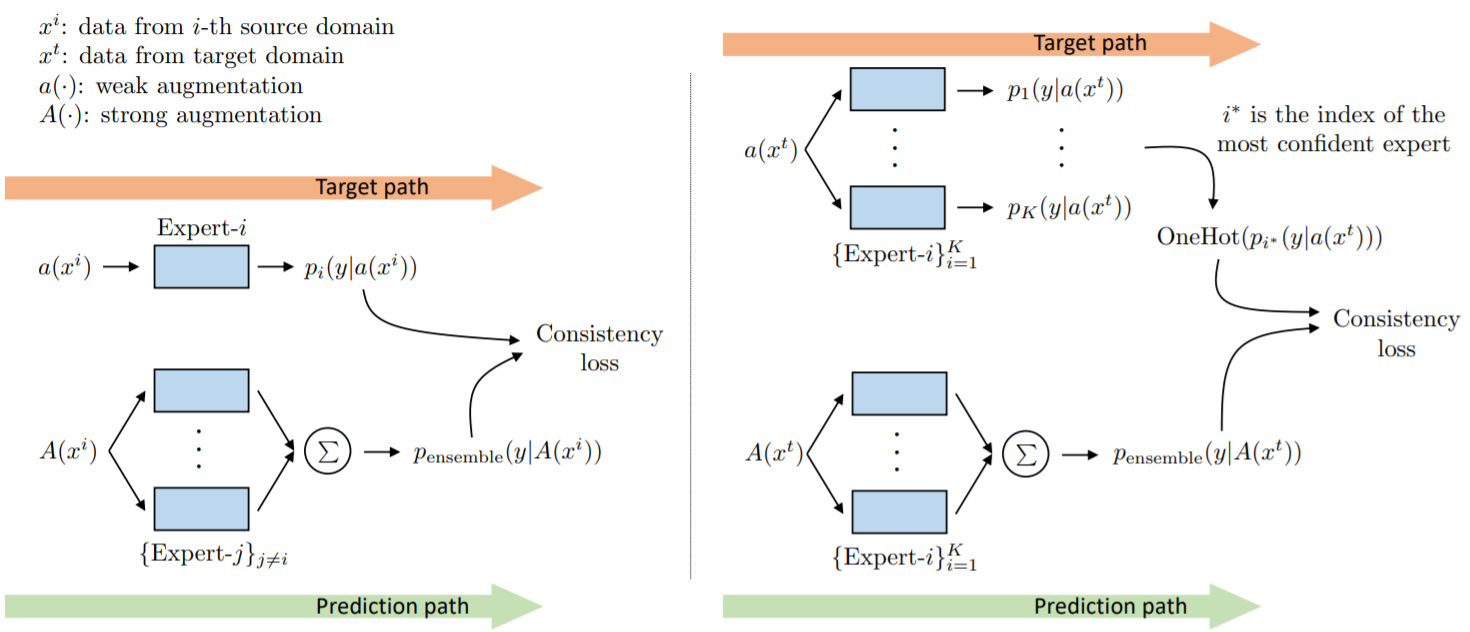
\includegraphics[scale=0.33]{20200927_DAEL.png}
    \caption{DAEL 框架:左图为 UDA 和 DG 的训练过程(无 target sample),右图为 UDA 的训练过程(有 target sample)}
    \label{fig:DAEL}
\end{figure}

\subsubsection{数据增强}

使用两种数据增强,weak 和 strong,分别用 $a(\cdot)$ 和 $A(\cdot)$ 表示,其中 weak 进行随机的翻转和偏移操作,strong 进行随机的噪声、旋转、锐化等操作。
如图 \ref{fig:DAEL} 所示,训练时 target path 使用 weak,prediction path 使用 strong。

\subsubsection{域特化的 expert 学习}

相当于是为每个 source 分类器(expert)建立对应的交叉熵损失:

$$
\mathcal{L}_{ce}=\frac{1}{K} \sum_{i=1}^{K} \mathbb{E}_{x^{i}, y\left(x^{i}\right) \sim \mathcal{D}_{i}}\left[H\left(y\left(x^{i}\right), E_{i}\left(a\left(x^{i}\right)\right)\right]\right.
$$

\subsubsection{使用 source data 的协作性 ensemble learning}

论文新提出的内容,使用 source sample 进行各个 expert 的协作学习,对于每一个 expert (当作是 pseudo-target-domain,使用 weak 数据增强),计算其与其它 expert (使用 strong 数据增强)的 consistency loss,
取平均后求和作为 collaborative ensemble learning 的损失:

$$
\mathcal{L}_{cr}=\frac{1}{K} \sum_{i=1}^{K} \mathbb{E}_{x^{i} \sim \mathcal{D}_{i}}\left[\left\|E_{i}\left(a\left(x^{i}\right)\right)-\frac{1}{K-1} \sum_{j \neq i} E_{j}\left(A\left(x^{i}\right)\right)\right\|^{2}\right]
$$

\subsubsection{使用 target sample 的协作性 ensemble learning}

论文新提出的内容,利用 target sample,使用所有 expert 生成 target 的 prediction $p_{i}(y|a(x^{t}))=E_{i}(a(x^{t}))$,
借助预测概率的最大值,选取最 confident 的 expert 的 prediction 作为 one-hot pseudo label $\arg \max (p_{i^{*}})$,
其中 $i^*$ 表示最 confident 的 expert 的 index $i^{*}=\arg \max ([\max(p_{1}), \ldots, \max(p_{K})])$。
接下来计算 strong 数据增强的 ensemble $\bar{E}(A(x^{t}))=\frac{1}{K} \sum_{i=1}^{K} E_{i}(A(x^{t}))$,利用交叉熵损失使其与前面得到的 one-hot pseudo label 相对应(fit)。
论文中还设置了一个预测概率的 threshold $\epsilon$ 来确保 pseudo 是比较可信的(即只有最大预测概率大于 $\epsilon$ 的结果才会参与这部分 loss 计算?):

$$
\mathcal{L}_{u}=\mathbb{E}_{x^{t} \sim \mathcal{D}_{T}}\left[\mathbf{1}\left(\max \left(p_{i^{*}}\right) \geq \epsilon\right) H\left(\hat{y}\left(x^{t}\right), \bar{E}\left(A\left(x^{t}\right)\right)\right)\right]
$$

当任务为 Domain Generalization 时(无 target sample),不计算这部分 loss。

模型的 objective function 如下:

$$
\mathcal{L}=\mathcal{L}_{c e}+\mathcal{L}_{c r}+\lambda_{u} \mathcal{L}_{u}
$$

\subsection{Experiments}

对于 MSDA,在 Digit-Five、DomainNet 和 miniDomainNet 上进行实验,结果如图 \ref{fig:UDA} 所示。

\begin{figure}[ht]
    \centering
    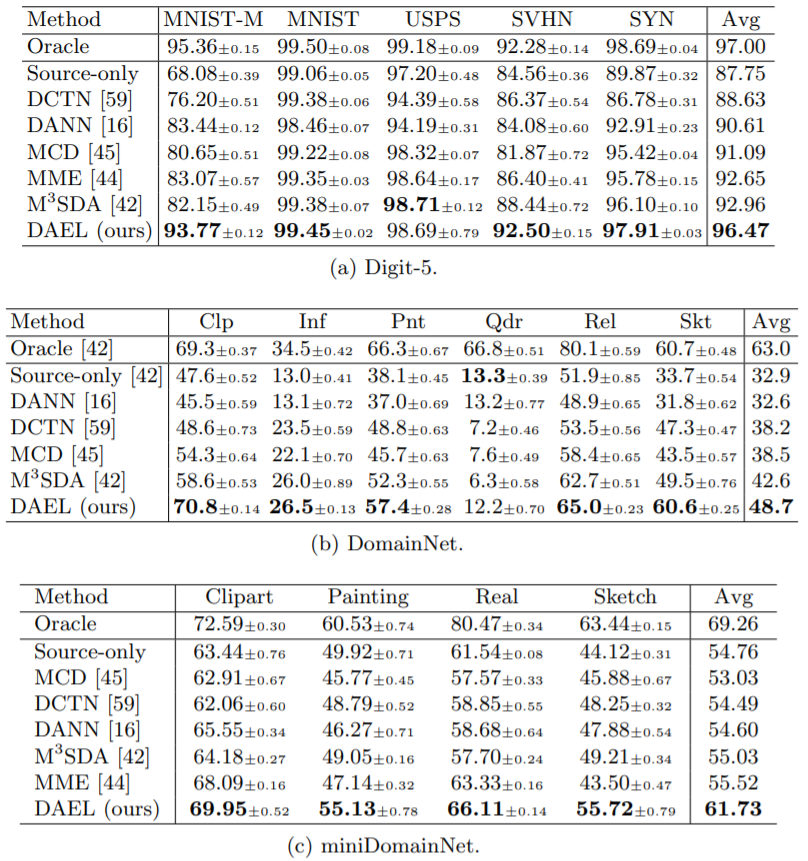
\includegraphics[scale=0.5]{20200927_Experiment_UDA.png}
    \caption{UDA 的实验结果}
    \label{fig:UDA}
\end{figure}

可以看到,论文提出的方法在多个 MSDA 数据集上都有非常明显的提升。

对于 DG,在 PACS 和 Office-Home 上进行实验,结果如图 \ref{fig:DG} 所示。

\begin{figure}[ht]
    \centering
    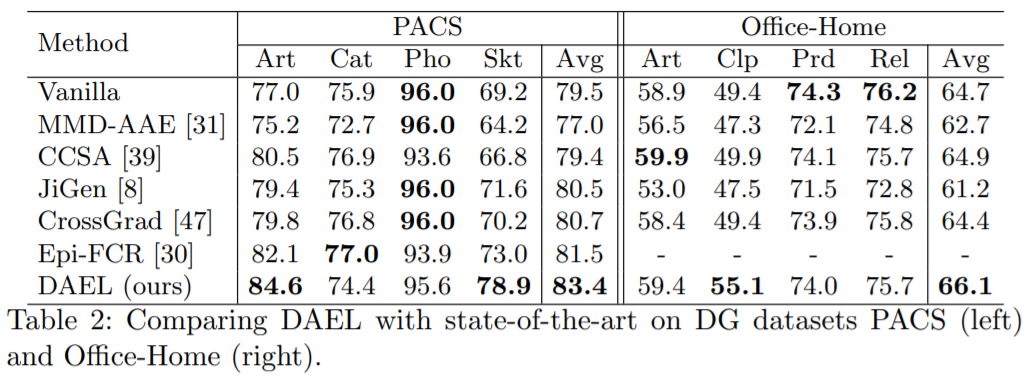
\includegraphics[scale=0.4]{20200927_Experiment_DG.png}
    \caption{DG 的实验结果}
    \label{fig:DG}
\end{figure}

\subsection{Analysis}

论文里做了很多方面的分析,包括消融实验、协作学习的作用、伪标签的生成、strong 数据增强的必要性等,这里列举一些比较重要的结果。

消融学习的结果如图 \ref{fig:Ablation} 所示,可以看到,新设计的两个 loss 都产生了作用,
其中作用比较明显的是使用 target sample 的协作学习损失,这也符合 MSDA 的假设,即利用 target sample 进行 domain adaptation。

\begin{figure}[ht]
    \centering
    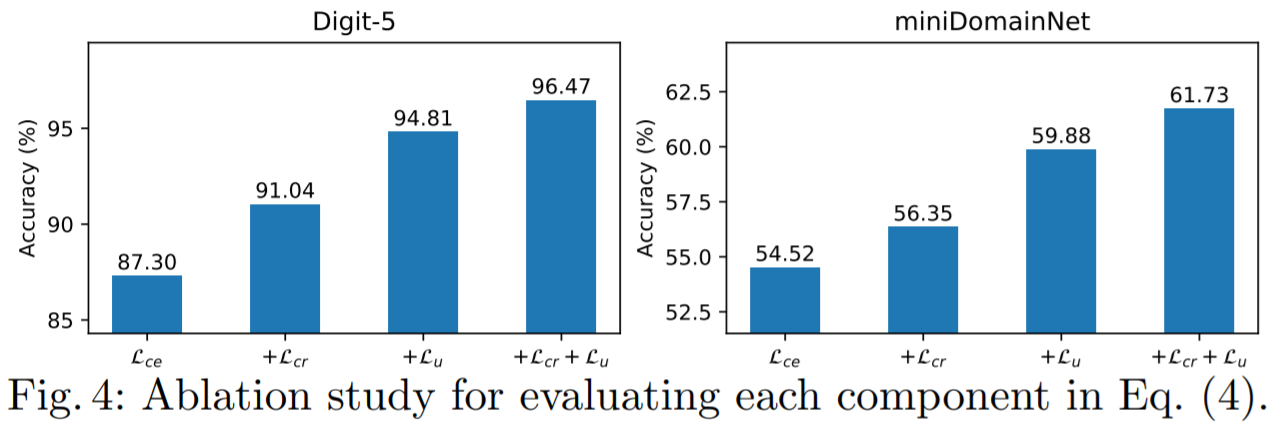
\includegraphics[scale=0.35]{20200927_Ablation.png}
    \caption{消融实验}
    \label{fig:Ablation}
\end{figure}

关于 $\mathcal{L}_{cr}$ 中应该使用 real label 还是 expert prediction 作为 supervise 的依据,
论文给出实验结果如图 \ref{fig:ER} 所示。发现 expert prediction 作为依据反而能得到略好一些的结果。

\begin{figure}[ht]
    \centering
    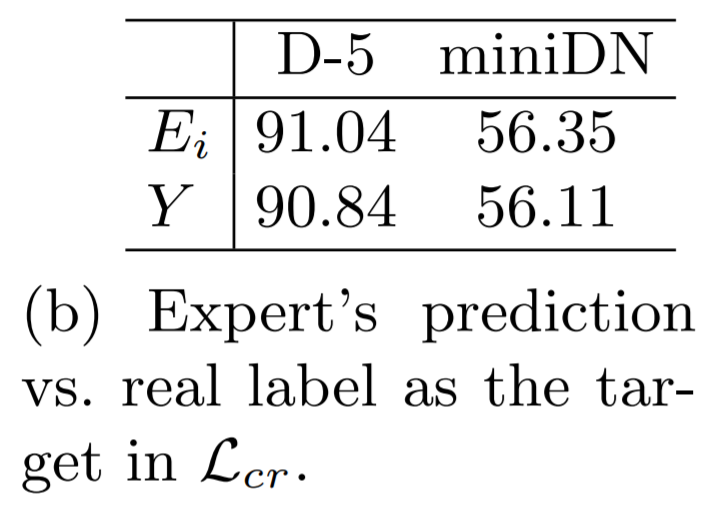
\includegraphics[scale=0.35]{20200927_Expert_Real.png}
    \caption{Real label 与 Expert prediction 对比}
    \label{fig:ER}
\end{figure}

关于数据增强的讨论,实验结果如图 \ref{fig:DataA} 所示。实验结果显示较强的数据增强措施可以比较好地剔除掉 corrupted pseudo label。

\begin{figure}[ht]
    \centering
    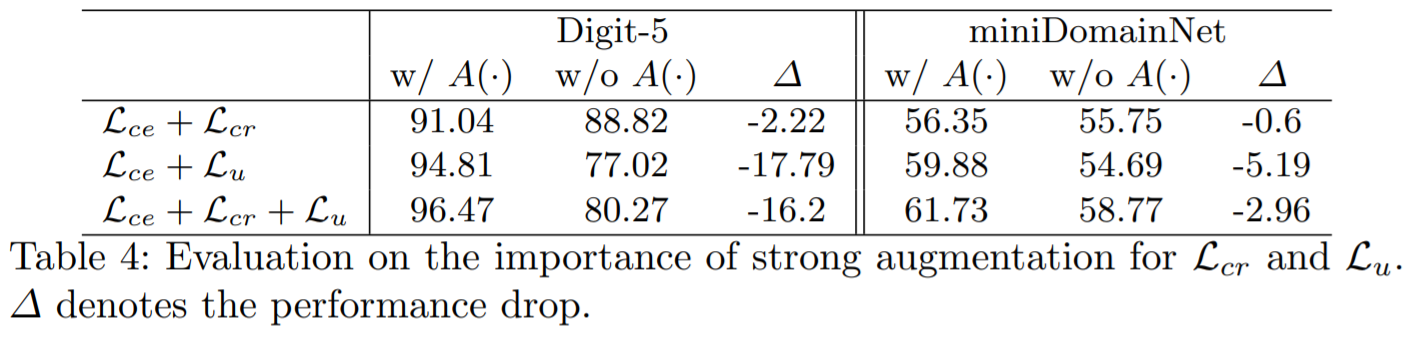
\includegraphics[scale=0.35]{20200927_DataA.png}
    \caption{不同数据增强(weak 和 strong)的作用}
    \label{fig:DataA}
\end{figure}

\section{值得借鉴的地方}

\begin{itemize}
    \item 多个 source domain 之间可以用一致性损失进行协作训练
    \item 用多个分类器去预测 target domain,选取预测概率最大的作为伪标签,概率大说明伪标签更可能是正确的
    \item 训练的时候设置一个预测概率的 threshold 来确保伪标签的可信度,可能可以解决前期伪标签不可信的问题(从某种角度上想相当于是做了 source distilling)
    \item 对于 source domain,训练的时候不一定要使用 real label 计算一致性损失,而可以选择使用不同分类器的预测结果作为 supervise 的依据
    \item 使用较强的数据增强措施剔除不好的 pseudo label
\end{itemize}

\end{document}
